% ==============================================================================
% SECCIÓN 2: PARTE 1 - DISEÑO DE HARDWARE  (versión ordenada)
% ==============================================================================
\section{Diseño de hardware}

% ------------------------------------------------------------------------------
\subsection{Diagrama de bloques funcionales y módulos de hardware}
% ------------------------------------------------------------------------------
La Figura~\ref{fig:bloques-funcionales} muestra los módulos de hardware elegidos para cada bloque funcional definido en el TP1 y la forma de comunicación entre ellos. La Tabla~\ref{tab:componentes} resume los componentes principales; su justificación se detalla en las secciones siguientes.

\begin{figure}[H]
    \centering
    \includegraphics[width=\linewidth]{imagenes/BloquesFuncionales-Hardware.png}
    \caption{Módulos de hardware utilizados en cada bloque funcional y forma de comunicación.}
    \label{fig:bloques-funcionales}
\end{figure}

\begin{table}[H]
\centering
\caption{Resumen de componentes principales.}
\label{tab:componentes}
\footnotesize
\begin{tabular}{L{3.1cm}L{4.1cm}L{3.0cm}L{2.2cm}}
\toprule
Componente & Código / valor & Formato físico & Bloque \\
\midrule
Motorreductor DC & GA12-N20, \SI{6}{V}--\SI{12}{V}, 150:1 & Motor con caja metálica & Tracción \\
Puente H doble & DRV8833  & Módulo & Tracción \\
Elevador de tensión & Módulo MT3608 & Módulo & Alimentación \\
Celda Li-ion & 18650, \SI{3,7}{V} & Cilíndrica & Alimentación \\
Portapilas & Uno para 1 celda 18650 y uno para 2 celdas 18650 en serie & Portapilas & Alimentación \\
Microcontrolador de prototipado & Arduino Nano & Módulo & Prototipo \\
Módulo WiFi & ESP32 DevKit v1 & Módulo & Comunicaciones \\
IMU & MPU6050 & Módulo & Sensado \\
Sensor de distancia ToF &  VL53L0X  & Módulo  & Sensado \\
Sensor magnético de ángulo &  AS5600 (TinyTronics AS5600MOD, SKU 004634), x2 & Módulo & Sensado \\
EDU-CIAA-NXP & LPC4337 & Placa & Procesamiento \\
\bottomrule
\end{tabular}
\end{table}


% ------------------------------------------------------------------------------
\subsection{Bloque de Sensado}
% ------------------------------------------------------------------------------
\subsubsection{Sensor de distancia: módulo VL53L0X}
La medición de distancia se realiza con un sensor de tiempo de vuelo (ToF) VL53L0X, en un módulo \emph{breakout} de cuatro pines (\texttt{VIN}, \texttt{GND}, \texttt{SCL}, \texttt{SDA}) \cite{vl53mod}, fijo sobre el chasis. Mide distancias de hasta \SI{2}{m} mediante un emisor láser de haz angosto, lo que lo hace adecuado para la detección precisa de obstáculos y permite resolver los límites del entorno con buena definición angular. El módulo incorpora un regulador de \SI{2,8}{V}, resistencias de \emph{pull-up} y capacitores, y puede alimentarse con \SI{2,6}{V} a \SI{5,5}{V}; su consumo según la hoja de datos es de \SI{10}{mA}. Se comunica por I\textsuperscript{2}C y los proveedores informan un rango de medición de \SI{30}{mm} a \SI{2000}{mm}.

\subsubsection{Sensor de ángulo de rueda: módulo AS5600}
Para estimar el giro de cada rueda se utilizan dos módulos AS5600 \cite{as5600mod}, uno por rueda. El AS5600 es un sensor magnético de posición angular absoluta de 12 bits (4096 posiciones por vuelta) con salidas I\textsuperscript{2}C, PWM y analógica. El módulo seleccionado funciona por defecto a \SI{3,3}{V}, tiene pines de paso \SI{2,54}{mm} e incluye un imán de magnetización diametral. Los detalles de montaje del imán y del módulo se describen en la Sección~\ref{sec:mecanica}.


% ------------------------------------------------------------------------------
\subsection{Bloque de Tracción y Actuación}
% ------------------------------------------------------------------------------
Según los requerimientos definidos en el TP1, este bloque debe contar con dos motores DC independientes para generar un movimiento diferencial, una rueda de apoyo auxiliar y un driver de potencia que module la energía provista por el subsistema de alimentación hacia los motores.

\subsubsection{Componentes y justificación}
\begin{itemize}[nosep]
  \item \textbf{Motores GA12-N20.} Se eligieron por: (i)~su tensión nominal de \SI{6}{V} a \SI{12}{V}, que permite alimentarlos desde dos celdas 18650 en serie (\SI{7,4}{V}) a través del puente H; (ii)~su baja velocidad con alto torque, gracias a la reducción de 150:1 con engranajes metálicos, adecuada para una plataforma que debe desplazarse lentamente y girar sobre su eje de manera controlada durante el escaneo; (iii)~su bajo consumo; (iv)~su tamaño y masa reducidos~\cite{ga12n20}. Sus características completas se resumen en la Tabla~\ref{tab:motor}.

  \item \textbf{Puente H DRV8833.} Es un puente H doble basado en transistores MOSFET de bajo consumo. De su hoja de datos se destacan: (i)~rango de tensión de alimentación de \SI{2,7}{V} a \SI{10,8}{V}, que cubre tanto una celda Li-ion (\SI{3,7}{V}) como dos celdas en serie (\SI{7,4}{V}); (ii)~corriente de \SI{1,5}{A} RMS y \SI{2,0}{A} de pico por puente H (uno por motor), superior a la corriente de bloqueo del motor; (iii)~protección térmica y contra baja tensión (UVLO); y (iv)~entradas compatibles con lógica de \SI{3,3}{V} y \SI{5}{V}.
\end{itemize}


\subsubsection{Características del motor GA12-N20}
\begin{table}[H]
\centering
\caption{Características del motor GA12-N20 (hoja de datos del fabricante, Handson Technology).}
\label{tab:motor}
\small
\begin{tabular}{L{6cm}L{5.5cm}}
\toprule
Parámetro & Valor \\
\midrule
Tensión nominal & \SI{6}{V}--\SI{12}{V} \\
Velocidad en vacío & \SI{50}{\rpm} a \SI{3}{V}; \SI{100}{\rpm} a \SI{6}{V}; \SI{200}{\rpm} a \SI{12}{V} \\
Velocidad con carga & \SI{80}{\rpm} \\
Torque nominal & \SI{2}{\kilo\gram\centi\meter} \\
Torque de bloqueo & \SI{3.4}{\kilo\gram\centi\meter} \\
Corriente nominal & \SI{0,07}{A} \\
Corriente de bloqueo & \SI{1}{A} \\
Relación de reducción & 1:150 \\
Engranajes & Metálicos \\
Dimensiones de la caja reductora & \SI{15}{mm}$\times$\SI{12}{mm}$\times$\SI{10}{mm} \\
Longitud total & \SI{34}{mm} \\
Eje de salida & \SI{3}{mm} de diámetro $\times$ \SI{10}{mm} de largo \\
Masa & \SI{10}{g} \\
\bottomrule
\end{tabular}
\caption{Características del motor GA12-N20 (hoja de datos del fabricante, Handson Technology~\cite{ga12n20}).}
\end{table}



\subsubsection{Condiciones de operación en el proyecto final}\label{sec:operacion}
En el prototipo los motores se alimentaron con aproximadamente \SI{4}{V}. En el proyecto final, el puente H entregará \SI{7,4}{V} (dos celdas en serie), pero los motores funcionarán con un ciclo de trabajo de aproximadamente el 50\,\%, de modo que la tensión media aplicada ($\approx$\SI{3,7}{V}) coincide aproximadamente con la utilizada en las pruebas. En consecuencia, los consumos medidos en el prototipo son representativos del funcionamiento final (Sección~\ref{sec:consumo-proto}).

\begin{visar}
La hoja de datos indica una variación lineal de la velocidad con la tensión (\SI{50}{RPM} por cada \SI{3}{V} aproximadamente). Con \SI{7,4}{V} y ciclo de trabajo máximo se estima una velocidad de $\approx$\SI{123}{RPM}; con ciclo de trabajo de $\approx$50\,\% (tensión media de \SI{3,7}{V}) resulta $\approx$\SI{62}{RPM}, similar a las $\approx$\SI{68}{RPM} esperables en el prototipo a \SI{4,08}{V}. Con ruedas de \SI{44}{mm} de diámetro, la velocidad lineal es
\begin{equation*}
v = \omega\, r = \frac{62 \cdot 2\pi}{60}\,\si{\radian\per\second} \times \SI{0,022}{m} \approx \SI{0,14}{\meter\per\second}
\end{equation*}
al 50\,\% de ciclo de trabajo, y de $\approx$\SI{0,28}{\meter\per\second} al máximo, lo que deja margen de regulación por PWM. La corriente nominal de \SI{0,07}{A} por motor es coherente con los $\approx$\SI{15}{mA} por motor medidos en vacío en el prototipo, ya que la corriente nominal corresponde a la condición de torque nominal.
\end{visar}

% ------------------------------------------------------------------------------
\subsection{Prototipado del subsistema de movimiento}
% ------------------------------------------------------------------------------
\subsubsection{Objetivos y componentes}
El prototipo se construyó con dos motores GA12-N20, un puente H DRV8833, un Arduino Nano como plataforma de prototipado para generar las señales de modulación por ancho de pulso (PWM) y una celda 18650 de \SI{3,7}{V}. El objetivo principal fue generar, desde el Arduino Nano, señales PWM hacia el puente H, de modo que éste aplique a cada motor la tensión requerida. Adicionalmente, se buscó adquirir conocimiento práctico sobre el comportamiento de los motores (fuerza, velocidad) y sobre el funcionamiento del DRV8833, con el fin de resolver con antelación los inconvenientes que pudieran surgir durante el ensamblaje del proyecto final.

\subsubsection{Configuración inicial de alimentación (prototipo 1)}
En una primera instancia, tanto el microcontrolador como los motores se alimentaron desde la misma celda de \SI{3,7}{V}, a través de un regulador elevador (\emph{step-up}) ajustado a \SI{6}{V}. Esta tensión se aplicó al pin \texttt{VIN} del Arduino Nano y al pin \texttt{VCC} del DRV8833 (Figura~\ref{fig:proto1}).

\begin{figure}[H]
    \centering
    \begin{subfigure}[b]{0.48\textwidth}
        \centering
        \includegraphics[width=\textwidth]{imagenes/Arturito_Prot_1a.png}
        \caption{}
    \end{subfigure}
    \hfill
    \begin{subfigure}[b]{0.48\textwidth}
        \centering
        \includegraphics[width=\textwidth]{imagenes/Arturito_Prot_1b.png}
        \caption{}
    \end{subfigure}
    \caption{Prototipo 1: una única celda de \SI{3,7}{V} con elevador de tensión a \SI{6}{V} alimenta tanto al Arduino Nano como al puente H DRV8833.}
    \label{fig:proto1}
\end{figure}

\subsubsection{Algoritmo de prueba}
Todas las pruebas se realizaron con un mismo algoritmo, consistente en un lazo infinito que ejecuta la secuencia de la Tabla~\ref{tab:secuencia}. El ciclo de trabajo (\emph{duty cycle}) se definió como variable global, con el fin de evaluar el efecto del PWM sobre el comportamiento de los motores. La espera de \SI{2}{s} entre acciones permite observar y medir el funcionamiento de los componentes. Para cada motor, el avance se logra con \texttt{IN1}~=~alto (PWM) e \texttt{IN2}~=~bajo, y el retroceso con \texttt{IN1}~=~bajo e \texttt{IN2}~=~alto (PWM).

\begin{table}[H]
\centering
\caption{Secuencia de movimientos del algoritmo de prueba.}
\label{tab:secuencia}
\begin{tabular}{clc}
\toprule
Etapa & Acción & Duración [s] \\
\midrule
1 & Espera & 2 \\
2 & Avanzar & 3 \\
3 & Espera & 2 \\
4 & Retroceder & 3 \\
5 & Espera & 2 \\
6 & Girar (primer sentido) & 3 \\
7 & Espera & 2 \\
8 & Girar (sentido contrario) & 3 \\
\bottomrule
\end{tabular}
\end{table}

\subsubsection{Problemas encontrados y resolución}

\paragraph{Pin de reposo (\texttt{nSLEEP}) del DRV8833.}
La primera prueba no resultó satisfactoria debido a que el DRV8833 dispone de un pin de reposo que debe mantenerse en nivel alto para que el controlador entregue tensión a los motores; de lo contrario, el dispositivo permanece en estado de bajo consumo (\emph{sleep}). Dado que en esta etapa no se requería dicho modo, se utilizó el puente de soldadura (\emph{jumper}) que provee el módulo para mantener este pin permanentemente en nivel alto. Una vez realizada esta corrección, el sistema funcionó correctamente.

\paragraph{Influencia de la tensión de alimentación.}
Se evaluó si el incremento de la tensión mediante el \emph{step-up} mejoraba la velocidad y el torque de los motores. A partir del análisis de la hoja de datos y de las características de la fuente disponible, se concluyó que, para este proyecto, la prioridad es el torque y no la velocidad.

\paragraph{Alimentación del Arduino Nano a través del pin \texttt{VIN}.}
Durante las pruebas se alimentó el Arduino Nano con \SI{5}{V} estables por el pin \texttt{VIN}. Dado que este pin se encuentra conectado a un regulador de tensión interno, la tensión efectiva de operación del microcontrolador resultó inferior a \SI{5}{V}, lo que provocó un comportamiento irregular y la imposibilidad de enviar correctamente las señales al puente H. Según la hoja de datos del Arduino Nano, la alimentación por \texttt{VIN} debe encontrarse entre \SI{6,5}{V} y \SI{12}{V}. Este resultado constituye una consideración relevante para el ensamblaje final: al alimentar la EDU-CIAA y el ESP32, deberá verificarse para cada pin de alimentación si existe un regulador intermedio, y definirse en consecuencia la tensión a suministrar.

\subsubsection{Configuración final de alimentación (prototipo 2)}
Con base en lo anterior, se optó por separar la alimentación de la parte lógica y la de potencia (motores), como muestra la Figura~\ref{fig:proto2}:

\begin{itemize}[nosep]
  \item \textbf{Lógica:} el Arduino Nano se alimentó por el pin \texttt{VIN} con una pila de \SI{9}{V}. La tensión en la alimentación del microcontrolador resultó de aproximadamente \SI{7}{V}, atribuible presumiblemente a la resistencia interna de la pila. Esta tensión permite que los pines de salida alcancen cómodamente el nivel alto de \SI{5}{V}.
  \item \textbf{Potencia:} la celda de litio, cargada a \SI{4,12}{V}, alimentó el DRV8833 con \SI{4,1}{V}, de modo que cada motor recibió \SI{4,08}{V} al máximo ciclo de trabajo.
\end{itemize}


La medición de \SI{7,1}{V} se realizó entre el pin \texttt{VIN} y \texttt{GND} del Arduino Nano, es decir, en la entrada del regulador lineal interno, antes de la regulación. La caída desde \SI{9}{V} se debe a la resistencia interna de la pila bajo carga (\emph{voltage sag}). A pesar de ello, la salida regulada (pin \texttt{5V}) entregó \SI{5,0}{V}, dado que \SI{7,1}{V} supera el umbral mínimo de entrada de \SI{6,5}{V}.


Con esta configuración el prototipo funcionó de manera estable y eficiente.

\begin{figure}[H]
    \centering
    \includegraphics[width=0.6\textwidth]{imagenes/Arturito_Prot_2a.png}
    \caption{Prototipo 2: el Arduino Nano se alimenta con una pila de \SI{9}{V} y el ramal de potencia (DRV8833 y motores) con una celda de \SI{3,7}{V} cargada a \SI{4}{V}.}
    \label{fig:proto2}
\end{figure}

\subsubsection{Ensayos de consumo}\label{sec:consumo-proto}
Se midieron la tensión y la corriente consumida por el prototipo con el objetivo de estimar el consumo del sistema final. La Tabla~\ref{tab:consumo} resume la corriente demandada por los \textbf{dos motores en conjunto} desde la celda de litio (en vacío, aproximadamente \SI{15}{mA} por motor). El Arduino Nano, alimentado con la pila de \SI{9}{V}, consumió entre \SI{19}{mA} y \SI{25}{mA}.

\begin{table}[H]
\centering
\caption{Consumo de corriente de ambos motores en simultáneo (alimentación \SI{4,1}{V}).}
\label{tab:consumo}
\begin{tabular}{lc}
\toprule
Condición de carga & Corriente [mA] \\
\midrule
En vacío (sin carga) & 30 \\
Ligeramente frenados & 60 \\
Ruedas frenadas, sin llegar a inmovilizarse (máximo) & 200 \\
\bottomrule
\end{tabular}
\end{table}

Como se explicó en la Sección~\ref{sec:operacion}, estos valores son representativos del funcionamiento final. Con modulación PWM, la corriente media del motor es aproximadamente la misma que con la tensión continua equivalente, mientras que la corriente tomada de la batería es del orden del ciclo de trabajo por la corriente del motor ($I_{\text{bat}} \approx D \cdot I_{\text{motor}}$), ya que la potencia se conserva ($\SI{3,7}{V} \cdot I_{\text{motor}} \approx \SI{7,4}{V} \cdot I_{\text{bat}}$). Con $D \approx 0{,}5$, los \SI{30}{mA}, \SI{60}{mA} y \SI{200}{mA} de la Tabla~\ref{tab:consumo} equivalen a $\approx$\SI{15}{mA}, \SI{30}{mA} y \SI{100}{mA} tomados de las celdas.

% ------------------------------------------------------------------------------
\subsection{Alimentación del sistema y elección de la fuente}
% ------------------------------------------------------------------------------
\subsubsection{Descarte de la pila de 9 V}
A partir de los resultados anteriores, y considerando las hojas de datos de la EDU-CIAA y del ESP32 con comunicación WiFi, se concluyó que la pila de \SI{9}{V} no resulta adecuada para el proyecto final, ya que presenta desgaste y caída de tensión durante la descarga.


Se utilizó una pila alcalina de \SI{9}{V} en formato PP3 (6F22/6LR61). Su capacidad nominal es de \SI{400}{\mAh} a \SI{500}{\mAh} con corrientes muy bajas, pero debido a su alta resistencia interna, con consumos continuos superiores a \SI{50}{mA} su capacidad útil se reduce a aproximadamente \SI{250}{\mAh}--\SI{350}{\mAh}. Con un consumo conjunto de la EDU-CIAA y el ESP32 de \SI{350}{mA}--\SI{550}{mA}, la autonomía resultaría de entre $250/550 \approx 0{,}45$~h y $350/350 = 1$~h.


\subsubsection{Consumos de cada bloque}
La Tabla~\ref{tab:balance} presenta el balance de consumo estimado del sistema final, con dos ramales de alimentación: lógica (referida a \SI{5}{V}) y potencia (motores).

\begin{table}[H]
\centering
\caption{Balance de consumo estimado del sistema final.}
\label{tab:balance}
\small
\begin{tabular}{L{4.6cm}cccc}
\toprule
Bloque & Ramal & Tensión [V] & $I_{\min}$ [mA] & $I_{\max}$ [mA] \\
\midrule
 EDU-CIAA-NXP (LPC4337) & Lógica & 5 & 180 & 320 \\
 ESP32 DevKit v1 (WiFi activo) & Lógica & 5 & 160 & 240 \\
 Módulo VL53L0X & Lógica & 3,3 & 10 & 20 \\
 Módulos AS5600 (x2) & Lógica & 3,3 & 26 & 26 \\
 IMU (MPU6050) & Lógica & 3,3 & 5 & 5 \\
\midrule
\textbf{Total ramal de lógica (referido a \SI{5}{V})} & & & \textbf{381} & \textbf{611} \\
\midrule
 Motores GA12-N20 (x2), corriente de batería & Potencia & 7,4 (PWM $\approx$50\,\%) & 30 & 200 \\
\bottomrule
\end{tabular}
\end{table}

\subsubsection{Arquitectura de alimentación}
El sistema se alimenta mediante dos ramales independientes con masa común:
\begin{itemize}[nosep]
  \item \textbf{Ramal de potencia (puente H DRV8833 y motores):} un portapilas con dos celdas 18650 en serie (\SI{7,4}{V} nominales, hasta \SI{8,4}{V} cargadas), dentro del rango de alimentación del DRV8833 (\SI{2,7}{V}--\SI{10,8}{V}). La velocidad de los motores se regula por PWM, con un ciclo de trabajo de operación del orden del 50\,\%.
  \item \textbf{Ramal de lógica (EDU-CIAA, ESP32 y sensores):} una única celda 18650 de \SI{3,7}{V} y un módulo elevador MT3608 ajustado a \SI{5}{V}, que mantiene una tensión estable independientemente de la descarga de la celda. La salida de \SI{5}{V} alimenta el pin de \SI{5}{V} de la EDU-CIAA y el pin \texttt{5V/VIN} del ESP32 DevKit, delegando la conversión a \SI{3,3}{V} en los reguladores internos de cada placa. Los sensores se alimentan a \SI{3,3}{V} desde las placas.
\end{itemize}

\subsubsection{Estimación de autonomía del ramal de lógica}
Con una celda de \SI{2200}{mAh}, la energía almacenada es
\begin{equation*}
E_{\text{bat}} = \SI{2,2}{Ah} \times \SI{3,7}{V} \approx \SI{8,14}{Wh}.
\end{equation*}
La potencia consumida a \SI{5}{V} (Tabla~\ref{tab:balance}) y la potencia tomada de la celda, suponiendo una eficiencia del elevador $\eta = 0{,}85$, son
\begin{align*}
P_{\min} &= \SI{5}{V} \times \SI{0,368}{A} = \SI{1,84}{W} \;\Rightarrow\; P_{\text{bat}} \approx \SI{2,17}{W},\\
P_{\max} &= \SI{5}{V} \times \SI{0,598}{A} \approx \SI{2,99}{W} \;\Rightarrow\; P_{\text{bat}} \approx \SI{3,52}{W}.
\end{align*}
La autonomía resulta entonces
\begin{equation*}
t_{\max} = \frac{\SI{8,14}{Wh}}{\SI{2,17}{W}} \approx \SI{3,8}{h}, \qquad
t_{\min} = \frac{\SI{8,14}{Wh}}{\SI{3,52}{W}} \approx \SI{2,3}{h},
\end{equation*}
con una corriente tomada de la celda de \SI{0,59}{A} a \SI{0,95}{A}.

\textbf{Justificación.} El valor de \SI{2,3}{h} corresponde al caso en que todas las placas y sensores consumen simultáneamente su valor máximo de forma sostenida. Estos valores máximos son picos (por ejemplo, las ráfagas de transmisión WiFi del ESP32 y la actividad plena de los periféricos de la EDU-CIAA), por lo que en funcionamiento normal el consumo medio será inferior y se ubicará más cerca del extremo inferior, con lo que la autonomía real será mayor. Aun descontando un 30\,\% de la capacidad nominal por la capacidad útil de la celda, el peor caso es de $\approx$\SI{1,6}{h}. Para un proyecto de carácter académico, en el que las pruebas, las demostraciones y las corridas de mapeo duran del orden de minutos y la celda puede recargarse o reemplazarse entre sesiones, esta autonomía resulta suficiente.

\subsubsection{Estimación de autonomía del ramal de potencia}
Con dos celdas en serie ($\approx$\SI{16,3}{Wh}) y una corriente de batería de \SI{100}{mA} a \SI{7,4}{V} ($\approx$\SI{0,74}{W}), la autonomía del ramal de potencia es de $\approx$\SI{22}{h}. En el peor caso, con los motores bloqueados de manera continua y una corriente de batería de \SI{0,62}{A} ($\approx$\SI{4,6}{W}), la autonomía sería de $\approx$\SI{3,5}{h}. En ambos casos el ramal de potencia no es el factor limitante frente al ramal de lógica.

\subsubsection{Protección y carga de las celdas}
Aún no se definieron la protección de las celdas ni el cargador.
\pendiente{definir el sistema de protección y el cargador, y reflejarlos en la lista de materiales.}

% ------------------------------------------------------------------------------
\subsection{Interfaces eléctricas entre bloques}
% ------------------------------------------------------------------------------
\subsubsection{Interfaz EDU-CIAA -- DRV8833}
El DRV8833 se controla mediante cuatro entradas lógicas (\texttt{IN1}--\texttt{IN4}), dos por cada puente H (uno por motor), compatibles con la lógica de \SI{3,3}{V} de la EDU-CIAA.

\begin{table}[H]
\centering
\caption{Control de un motor mediante las entradas del puente H.}
\label{tab:logica}
\begin{tabular}{lcc}
\toprule
Acción & \texttt{IN1} & \texttt{IN2} \\
\midrule
Avance & Alto (PWM) & Bajo \\
Retroceso & Bajo & Alto (PWM) \\
\bottomrule
\end{tabular}
\end{table}
\pendiente{asignar los pines concretos de la EDU-CIAA (salidas PWM) a \texttt{IN1}--\texttt{IN4}.}

\subsubsection{Bus \texorpdfstring{I\textsuperscript{2}C}{I2C} y salidas PWM de sensores}\label{sec:i2c}
El módulo VL53L0X y la IMU MPU6050 se comunican por I\textsuperscript{2}C (Tabla~\ref{tab:i2c}). Dado que los dos módulos AS5600 comparten la misma dirección fija (\texttt{0x36}) y no se pueden reprogramar, las dos unidades AS5600 no pueden compartir el mismo bus. Para resolverlo se investigó la datasheet del LPC4337 donde se halló que existen dos interfaces de comunicación  I\textsuperscript{2}C pero la placa EDU-CIAA solo expone una de ellas. Sin embargo, al revisar el esquemático para ver si los pines dedicados del microcontrolador estaban expuestos para su uso, se encontró que efectivamente los pines que la placa EDU-CIAA expone como aptos para comunicacion mediante RS232 estan conectados directamente a los pines del microcontrolador para la segunda interfaz de I\textsuperscript{2}C. Todavia faltan realizar las pruebas para ver si esta opcion es viable, en caso contrario se implementaran las comunicaciones con los encoders mediante PWM por la salida OUT de los encoders y utilizando input capture desde la EDU-CIAA.

\begin{table}[H]
\centering
\caption{Dispositivos conectados al bus I\textsuperscript{2}C.}
\label{tab:i2c}
\small
\begin{tabular}{L{3.8cm}cL{5.6cm}}
\toprule
Dispositivo & Dirección (7 bits) & Observación \\
\midrule
Módulo VL53L0X & 0x29 & Una única unidad; el módulo expone solo 4 pines \\
IMU MPU6050 & 0x68 / 0x69 & Seleccionable con el pin \texttt{AD0} \\
\bottomrule
\end{tabular}
\end{table}

% ------------------------------------------------------------------------------
\subsection{Circuito esquemático}
% ------------------------------------------------------------------------------
\begin{visar}
\textbf{Criterios de modelado en KiCad.} Los módulos integrados (ESP32, DRV8833 y MT3608) se modelan como cajas negras mediante tiras de pines (\emph{pin headers}) de paso \SI{2,54}{mm}, conectando únicamente sus entradas y salidas.

\textbf{Componentes discretos de filtrado.}
\begin{itemize}[nosep]
  \item Un capacitor electrolítico de \SI{470}{\micro F}/\SI{16}{V} en paralelo con la alimentación de potencia del DRV8833 (pin \texttt{VM} a \texttt{GND}).
  \item Un capacitor cerámico de \SI{100}{nF} (código 104), soldado directamente en los bornes de cada motor, para filtrar el ruido de conmutación (EMI).
\end{itemize}
\end{visar}
\pendiente{Evaluar la adición de los componentes discretos de filtrado. Insertar el esquemático completo realizado en KiCad.}

% ------------------------------------------------------------------------------
\subsection{Diseño mecánico}\label{sec:mecanica}
% ------------------------------------------------------------------------------


% El [H] fuerza a que la imagen quede EXACTAMENTE debajo de \subsection
\begin{figure}[H]
	\centering
	% --- PRIMERA FILA: 2 imágenes grandes ---
	\begin{subfigure}[b]{0.48\textwidth}
		\centering
		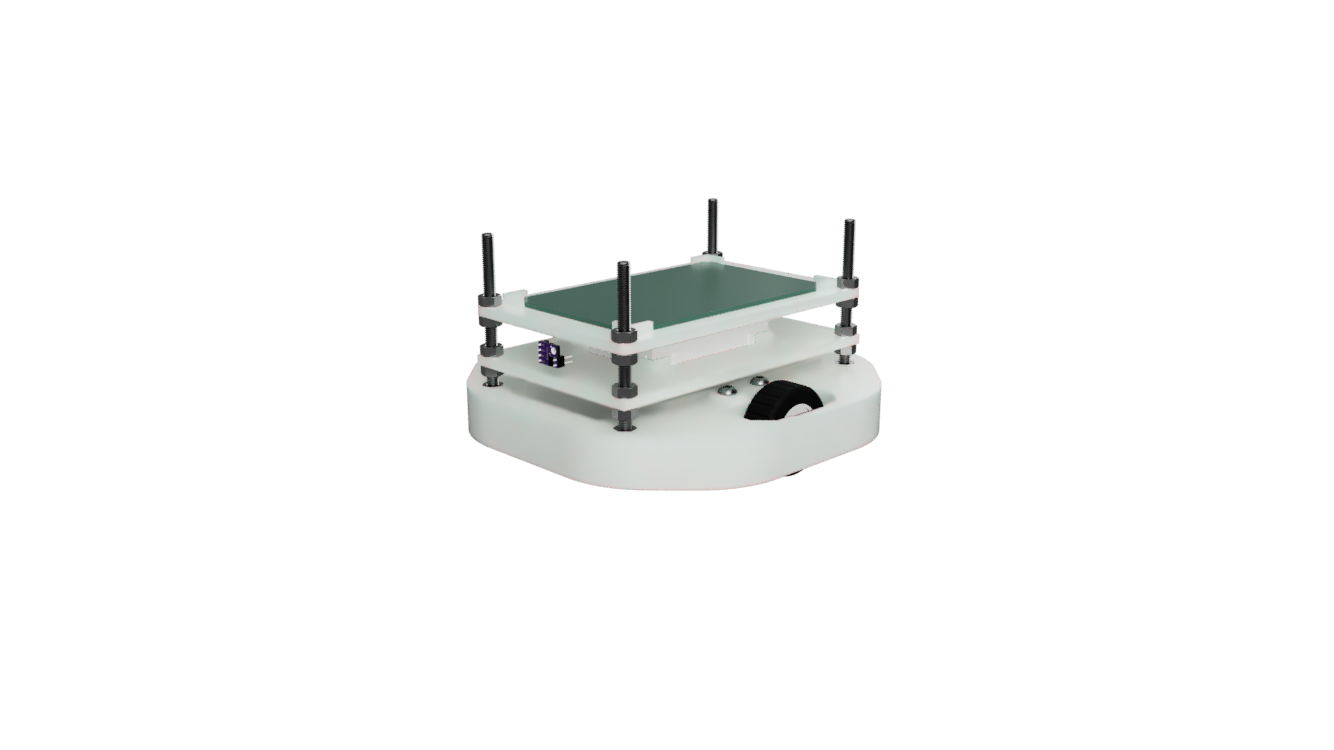
\includegraphics[width=\textwidth]{Imagenes/ArturitoMain.png}
		\caption{Modelo completo.}
		\label{fig:render_completo}
	\end{subfigure}
	\hfill
	\begin{subfigure}[b]{0.48\textwidth}
		\centering
		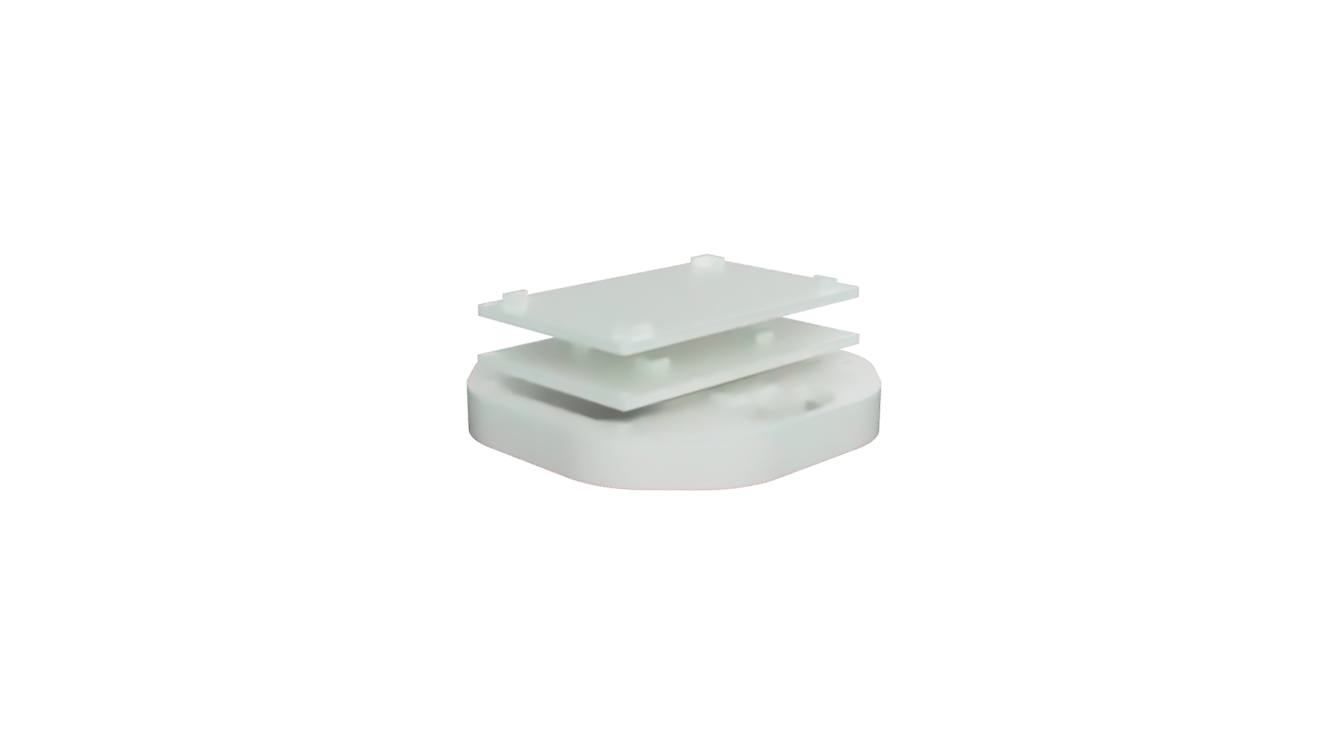
\includegraphics[width=\textwidth]{Imagenes/Impresion.png}
		\caption{Piezas impresas (ABS).}
		\label{fig:render_impresion}
	\end{subfigure}
	
	\vspace{0.3cm} % Espacio vertical entre la primera y segunda fila
	
	% --- SEGUNDA FILA: 1 imagen centrada ---
	\begin{subfigure}[b]{0.55\textwidth}
		\centering
		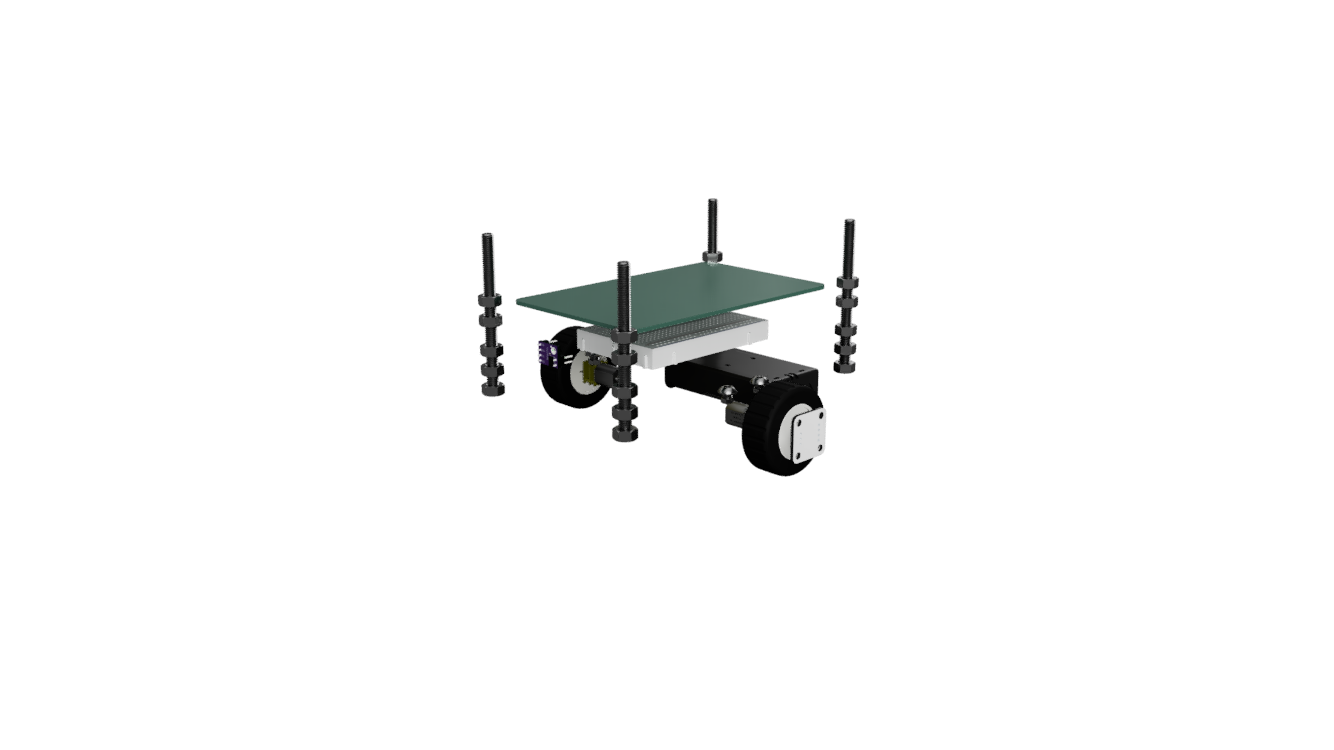
\includegraphics[width=\textwidth]{Imagenes/Referencias.png}
		\caption{Componentes/Hardware.}
		\label{fig:render_referencias}
	\end{subfigure}
	
	\caption{Desglose y vistas del modelo CAD paramétrico del chasis.}
	\label{fig:renders_chasis}
\end{figure}

\subsubsection{Arquitectura general y selección de materiales}
El chasis del robot se concibió bajo una filosofía de diseño modular y apilable en niveles, modelado de forma paramétrica en Autodesk Fusion. \pendiente{agregar el modelo CAD en un anexo o en la bibliografía.}
\begin{itemize}[nosep]
    \item \textbf{Proceso de manufactura:} impresión 3D por Fabricación por Filamento Fundido (FFF) en una impresora Creality Ender-3 S1.
    \item \textbf{Material:} ABS, por su resistencia mecánica y al impacto.
    \item \textbf{Unión de niveles:} la vinculación estructural vertical entre plataformas se resuelve mediante varillas roscadas y tuercas estandarizadas M3 y M6.
\end{itemize}

\subsubsection{Requisitos del chasis}

\pendiente{incorporar estos requisitos a la sección de requerimientos del TP1 si aún no figuran.}
\begin{itemize}[nosep]
    \item \textbf{Sensores de ángulo:} cada módulo AS5600 debe quedar enfrentado a una rueda, con el imán de magnetización diametral pegado en el eje de la rueda y alineado con su eje de rotación.
    \item \textbf{Radio de giro:} el chasis debe permitir un radio de giro nulo (girar sobre su propio eje).
    \item \textbf{Sensor ToF:} el VL53L0X debe apuntar al frente, sobre el eje de simetría del chasis, con el campo de visión despejado durante el giro del robot.
    \item \textbf{Tracción:} el chasis debe poder desplazarse con los motores y ruedas disponibles.
    \item \textbf{Alimentación:} el chasis debe tener espacio para los dos sistemas de alimentación separados: un portapilas de una celda 18650 (lógica) y uno de dos celdas 18650 (potencia).
\end{itemize}

\subsubsection{Tracción y apoyo}
El sistema adopta una configuración cinemática de tracción diferencial, con dos motores GA12-N20 acoplados a ruedas de \SI{44}{mm} de diámetro. El portapilas de dos celdas se ubica en la sección posterior, para desplazar el centro de gravedad hacia el punto de apoyo. En la versión CAD actual el apoyo trasero aún no está diseñado: será un patín deslizante integrado e impreso en ABS que se ensayará en la siguiente fase de prototipado; si las pérdidas por fricción resultan elevadas, se lo reemplazará por una rueda de bolas de acero (\emph{ball caster}).

\subsubsection{Integración de sensores}
\begin{itemize}[nosep]
    \item \textbf{Módulos AS5600:} el chasis integra soportes enfrentados a cada rueda, con los ejes de rotación alineados. El imán se monta centrado en el extremo del eje de la rueda, con una separación respecto del sensor de entre \SI{1}{mm} y \SI{2}{mm}. Como el motor GA12-N20 no tiene eje trasero accesible, el imán no puede montarse en el rotor y gira a la velocidad de la rueda ($\approx$\SI{62}{RPM}), lo que simplifica el conteo de vueltas.
    \item \textbf{Soporte del sensor ToF:} se ubica en el extremo frontal, sobre el eje de simetría del robot, para garantizar un campo de visión despejado. Su geometría se encuentra en etapa de finalización.
\end{itemize}


\begin{visar}
La cobertura de $360^\circ$ se obtiene haciendo girar el robot completo, por lo que el ángulo de cada medición proviene de la odometría (AS5600) y de la IMU. Conviene medir el desplazamiento del sensor ToF respecto del centro de giro (punto medio entre ruedas) para corregirlo en el cálculo del mapa. Dado que el robot gira apoyado en el patín, pueden producirse deslizamientos que degraden la estimación del ángulo solo con los AS5600; el giróscopo de la IMU permite compensarlo.

La resolución angular depende de la velocidad de giro $\omega$ y del tiempo de medición $T_s$ del sensor: $\Delta\theta = \omega\,T_s$. Con $T_s \approx \SI{33}{ms}$ y una muestra por grado, la velocidad máxima de giro es de $\approx 30\,^\circ/\mathrm{s}$ (una vuelta completa en $\approx\SI{12}{s}$).
\end{visar}


\subsubsection{Estado de fabricación y próximos pasos}
A la fecha de este informe, el diseño 3D se encuentra en fase de cierre en entorno CAD y aún no se inició la impresión de las piezas. Los próximos pasos son:
\begin{itemize}[nosep]
    \item \textbf{Pruebas de tolerancia:} impresión de piezas de prueba con distintas tolerancias para validar los encastres de las tuercas y varillas M3 y M6 antes de imprimir el chasis completo.
    \item \textbf{Impresión 3D e integración física:} Fabricación de los niveles y montaje de la electrónica.
    \item \textbf{Validación de Apoyo:} Evaluación experimental de la fricción del apoyo de ABS.
\end{itemize}

